\clearpage

\section {Systematic effects in the prediction of energy spectra}
\label{sec:systematics}

The description of the systematic parameters in this analysis can be found in \cite{OurRun18JointAnalysis3Flavour} (Sec. 3), this section will present the pre- and post-BANFF flux and cross-section covariance matrices and the SK detector covariance matrix and SK FSI, SI and PN covariance matrix. A summary of the best-fit values and pre- and post-BANFF errors of all systematics can be found in \cref{app:systematics}.

\begin{figure*}[htb]
	\center
	\begin{subfigure}[b]{0.49\textwidth}
		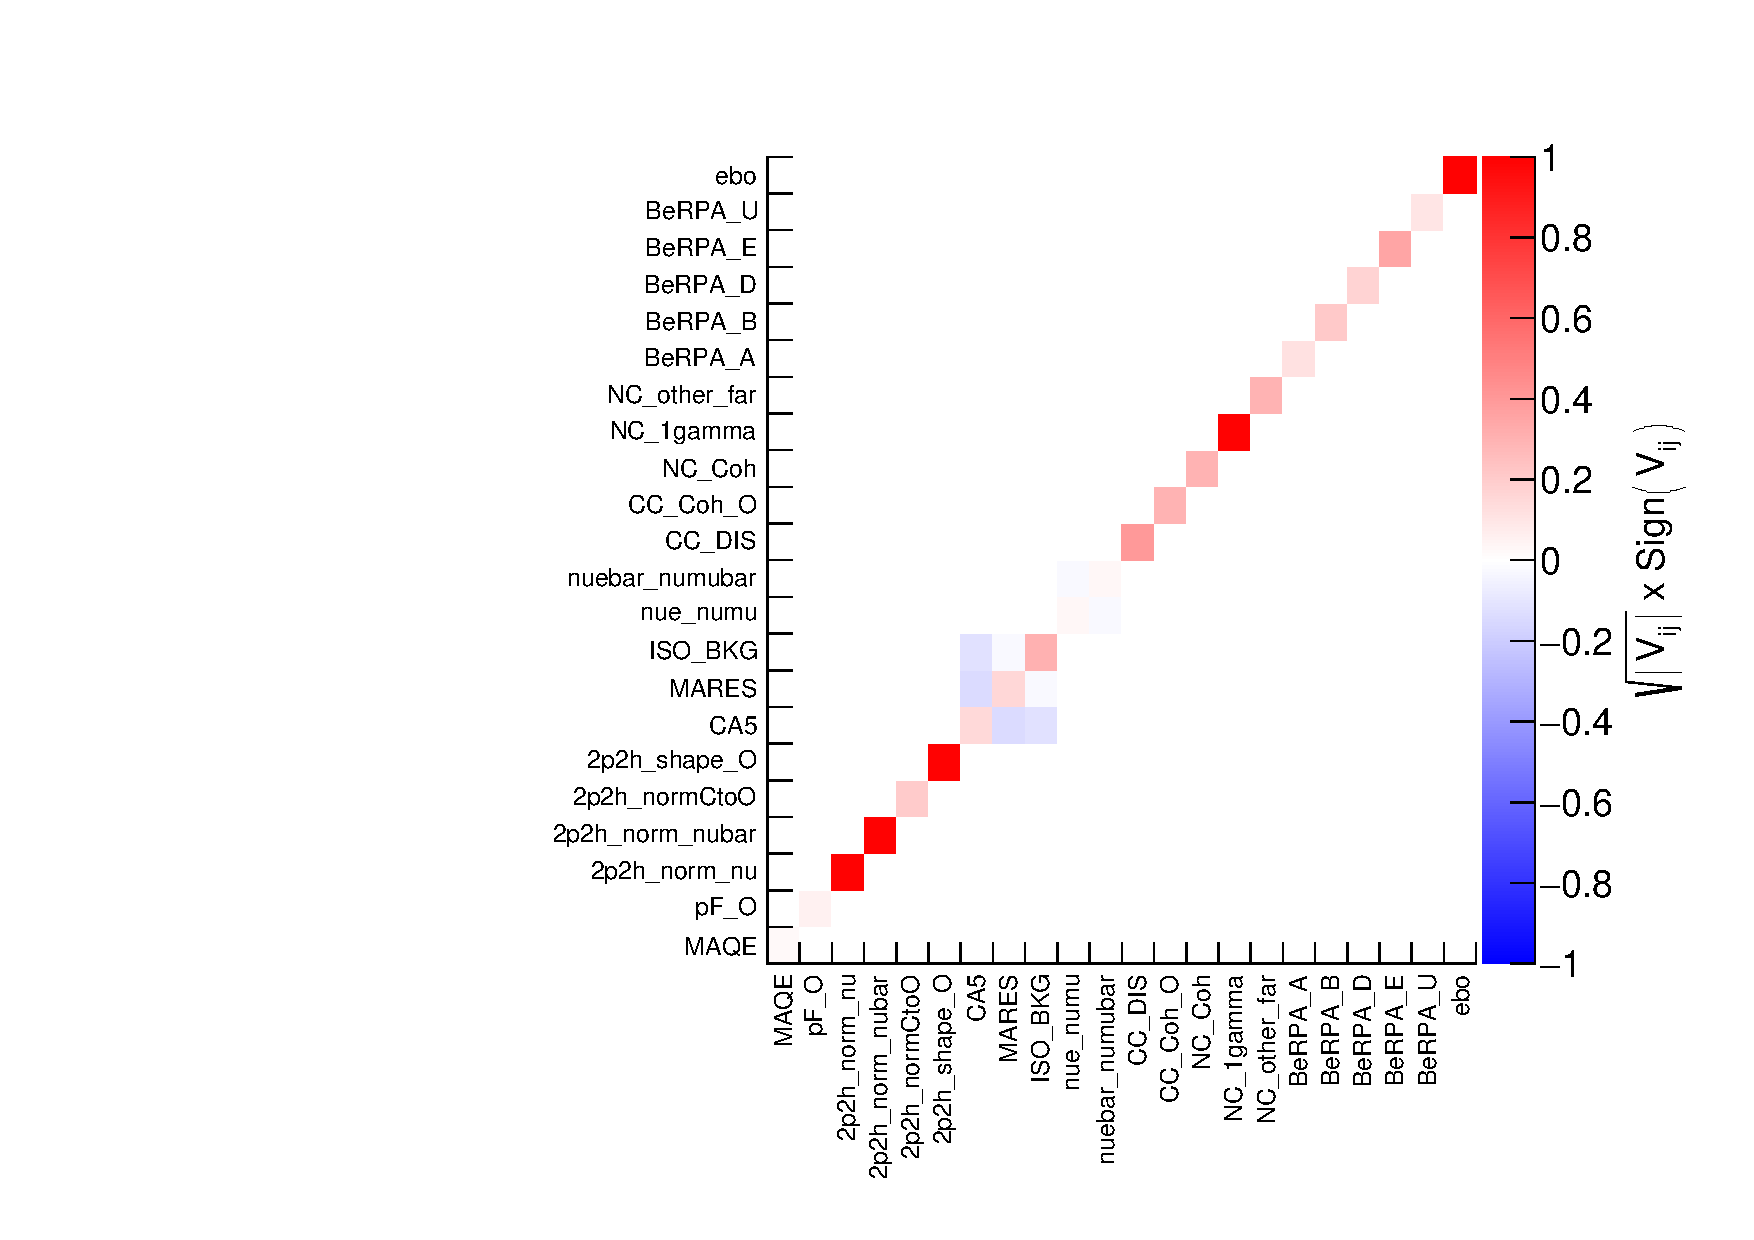
\includegraphics[width=\textwidth]{images/banff/xsec_prefit}
	\end{subfigure}
	\begin{subfigure}[b]{0.49\textwidth}
		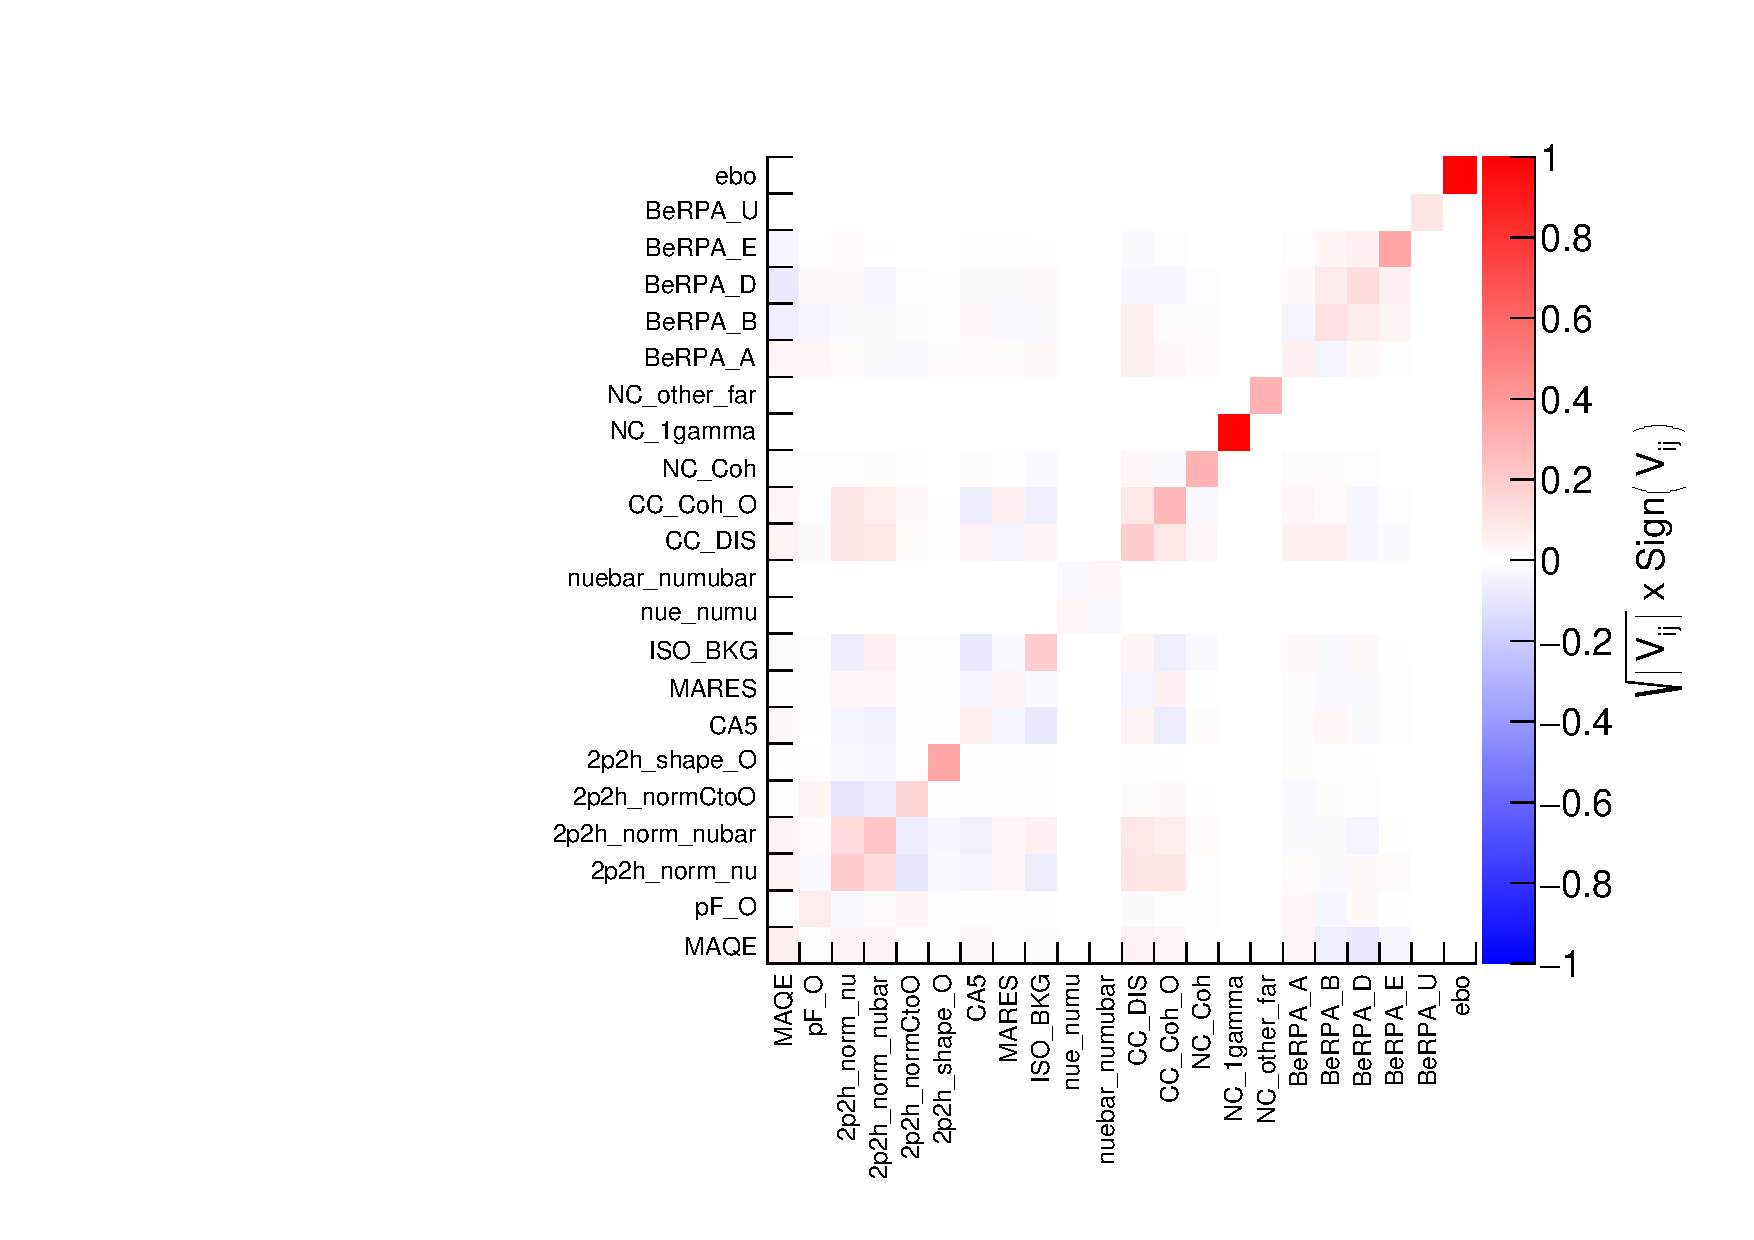
\includegraphics[width=\textwidth]{images/banff/xsec_postfit}
	\end{subfigure}
	\caption{The pre-BANFF (left) and post-BANFF (right) cross-section covariance matrix, with the values shown as the sign of the element times the square root of the absolute value of the element.}
	\label{fig:xsec_corr}
\end{figure*}

\begin{figure*}[htb]
	\center
	\begin{subfigure}[b]{0.7\textwidth}
		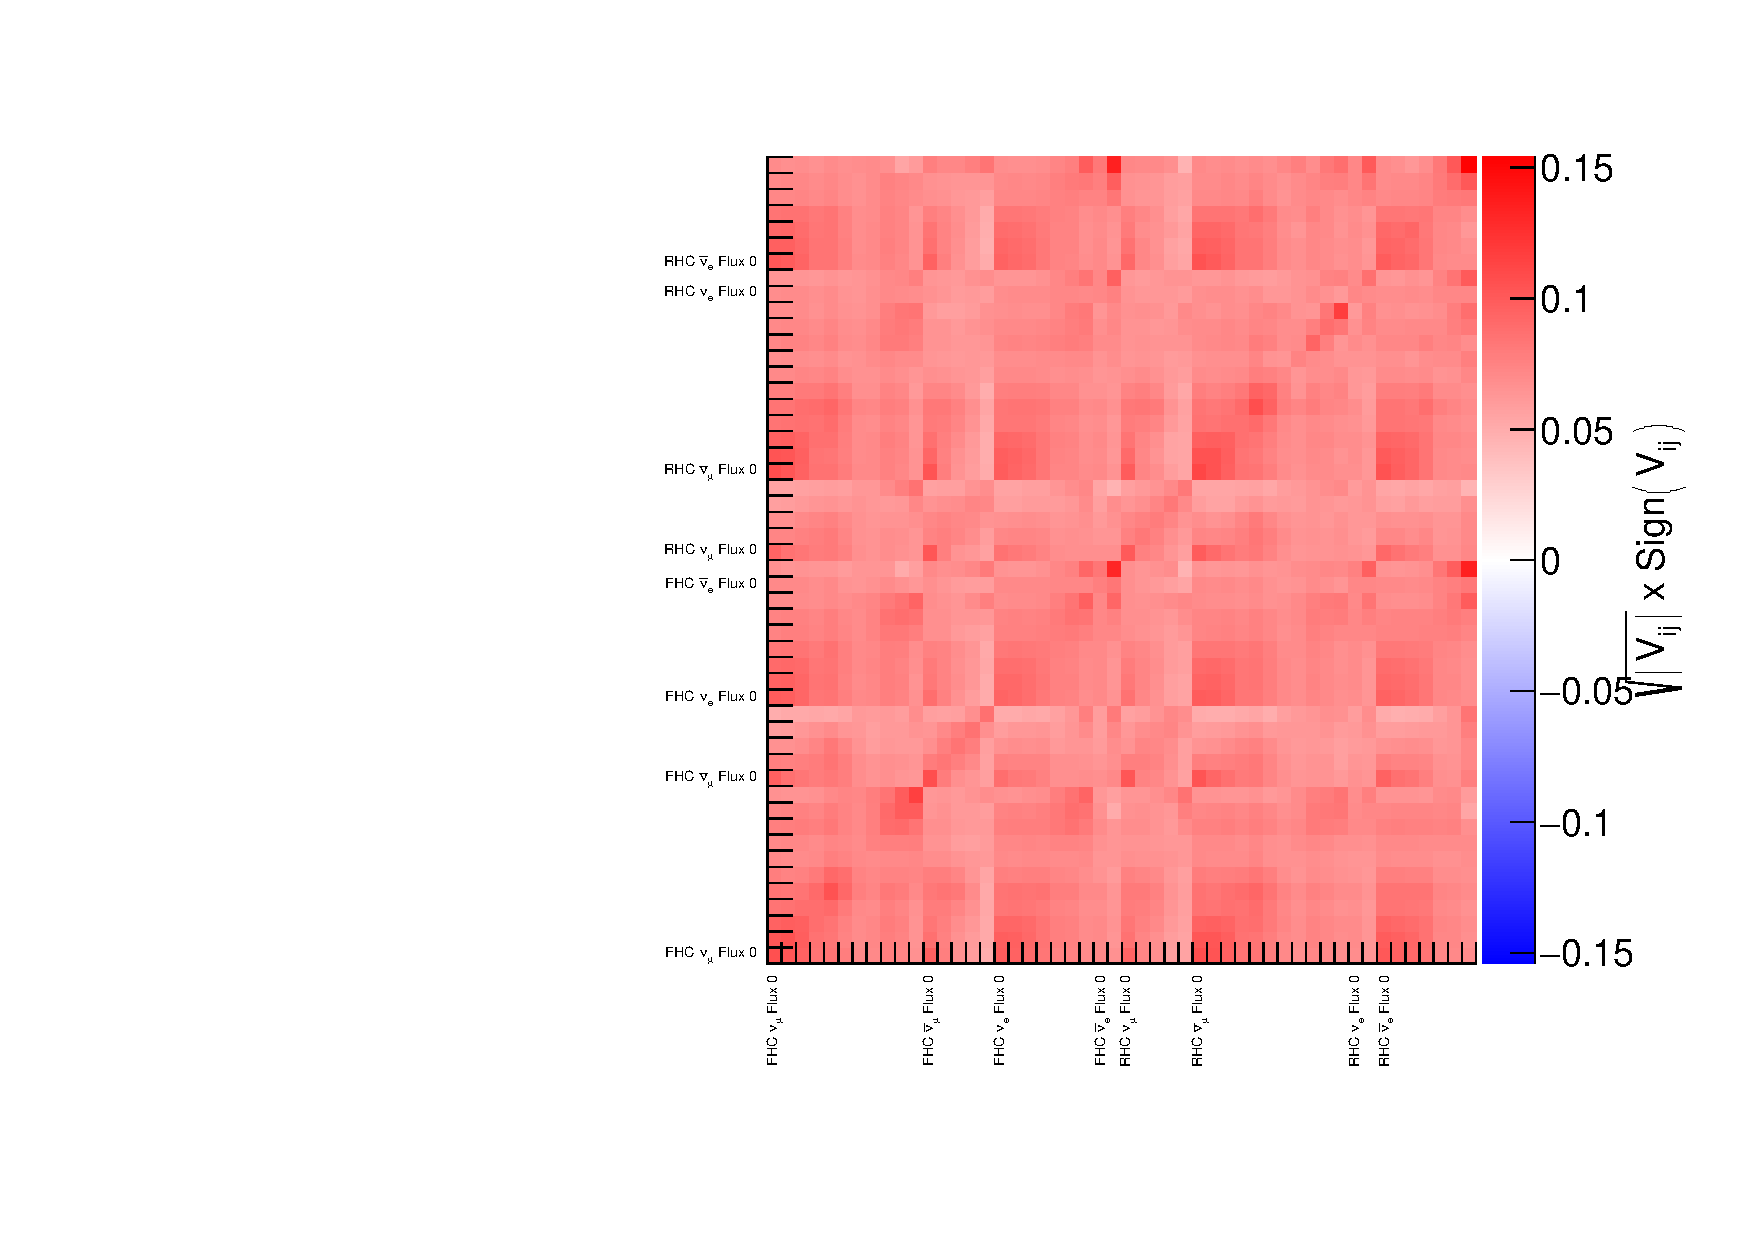
\includegraphics[width=\textwidth]{images/banff/flux_prefit}
	\end{subfigure}
	\begin{subfigure}[b]{0.7\textwidth}
		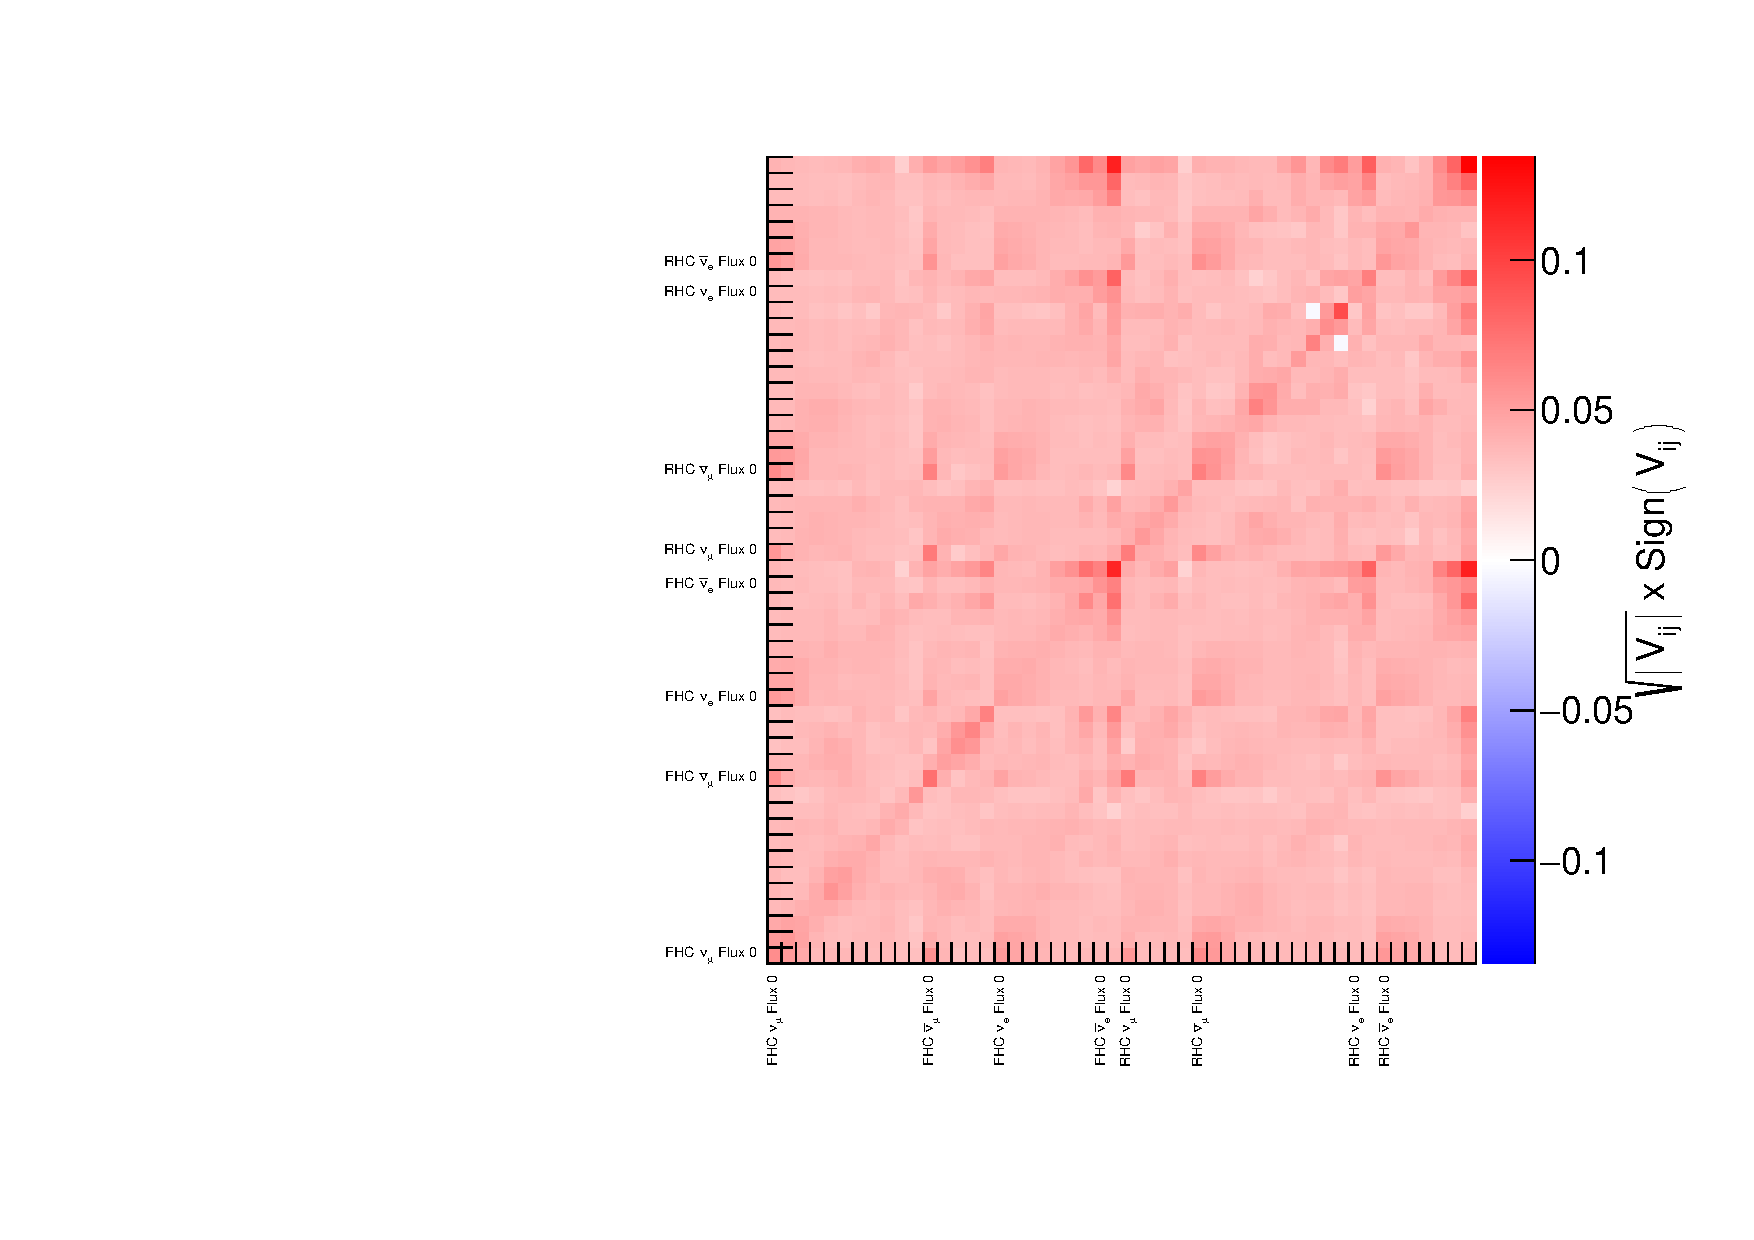
\includegraphics[width=\textwidth]{images/banff/flux_postfit}
	\end{subfigure}
	\caption{The pre-BANFF (top) and post-BANFF (bottom) flux covariance matrix, with the values shown as the sign of the element times the square root of the absolute value of the element.}
	\label{fig:flux_corr}
\end{figure*}

\begin{figure*}[htb]
	\center
	\begin{subfigure}[b]{0.7\textwidth}
		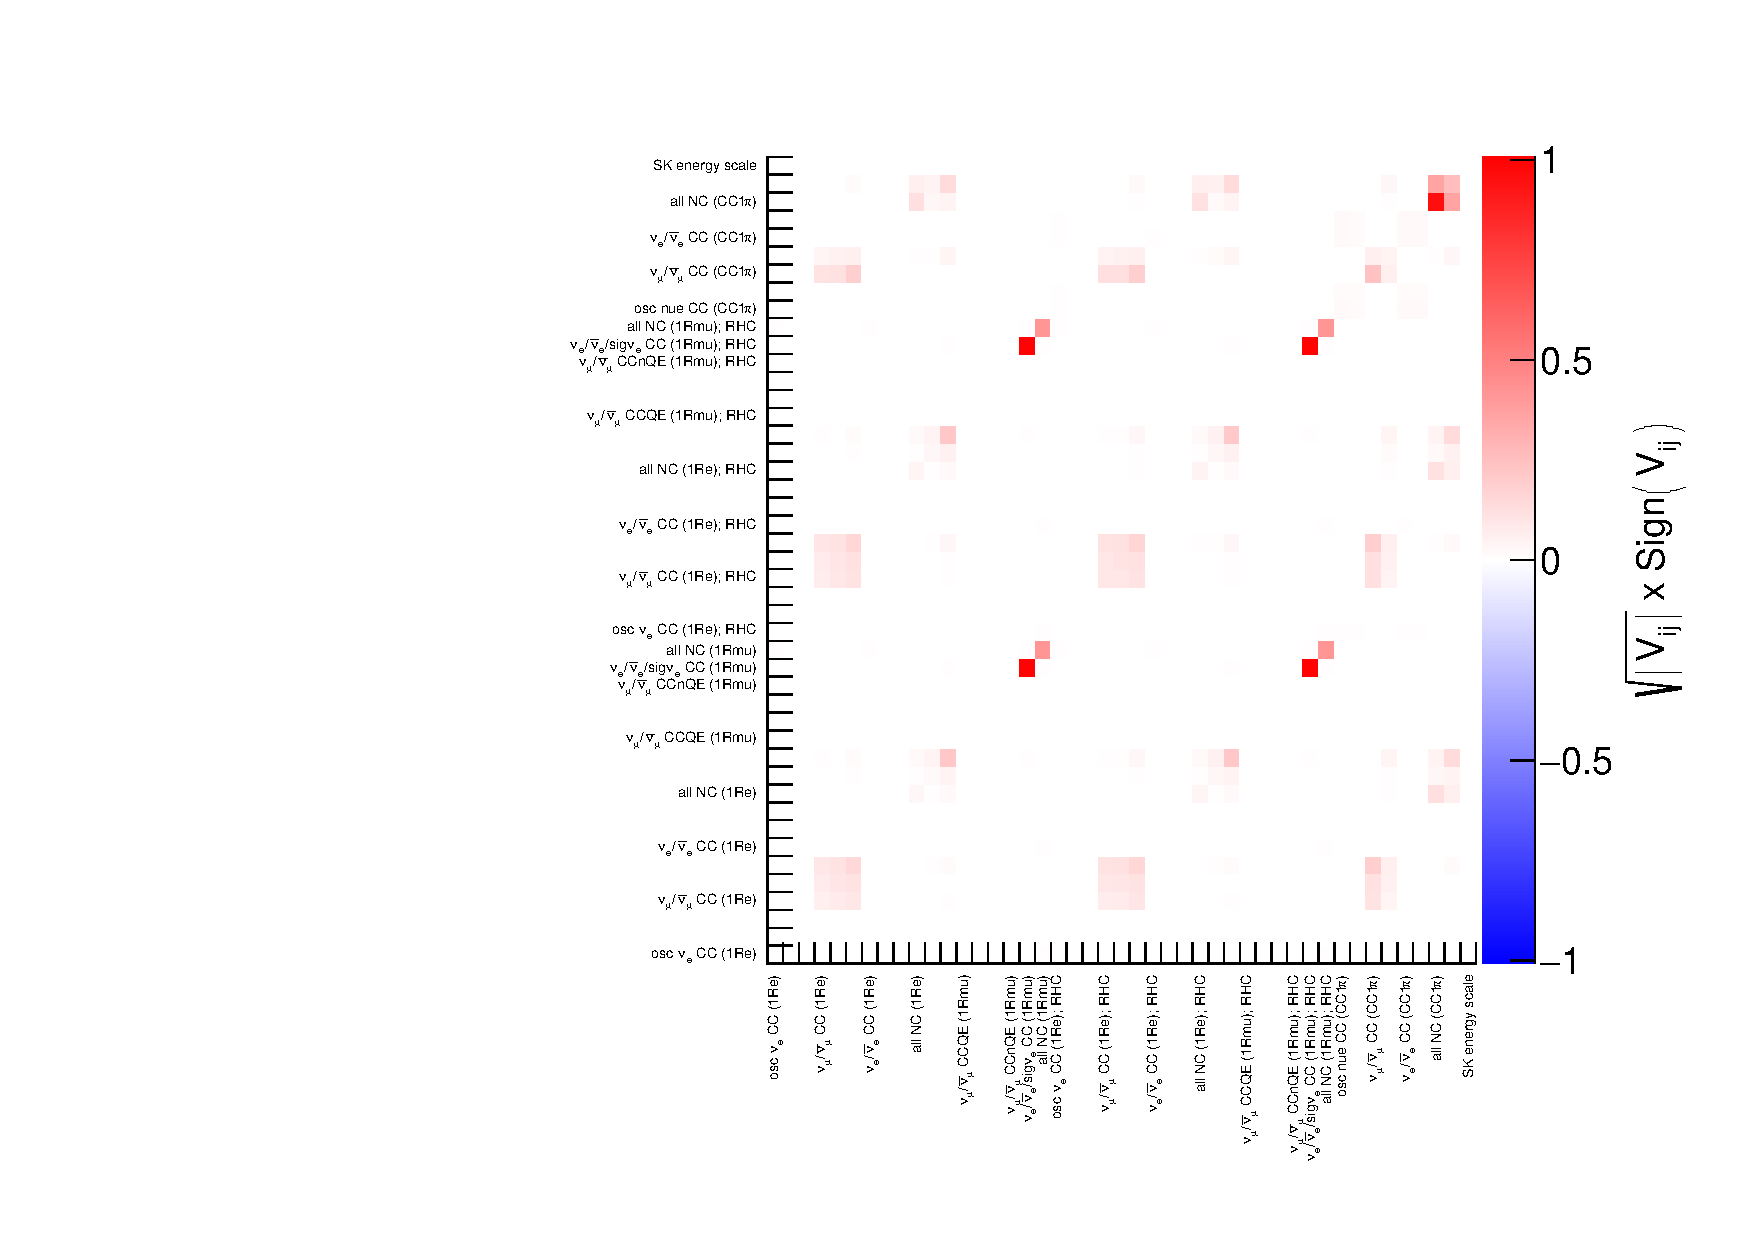
\includegraphics[width=\textwidth]{images/skdetfsi/skmatrix_det}
	\end{subfigure}
	\begin{subfigure}[b]{0.7\textwidth}
		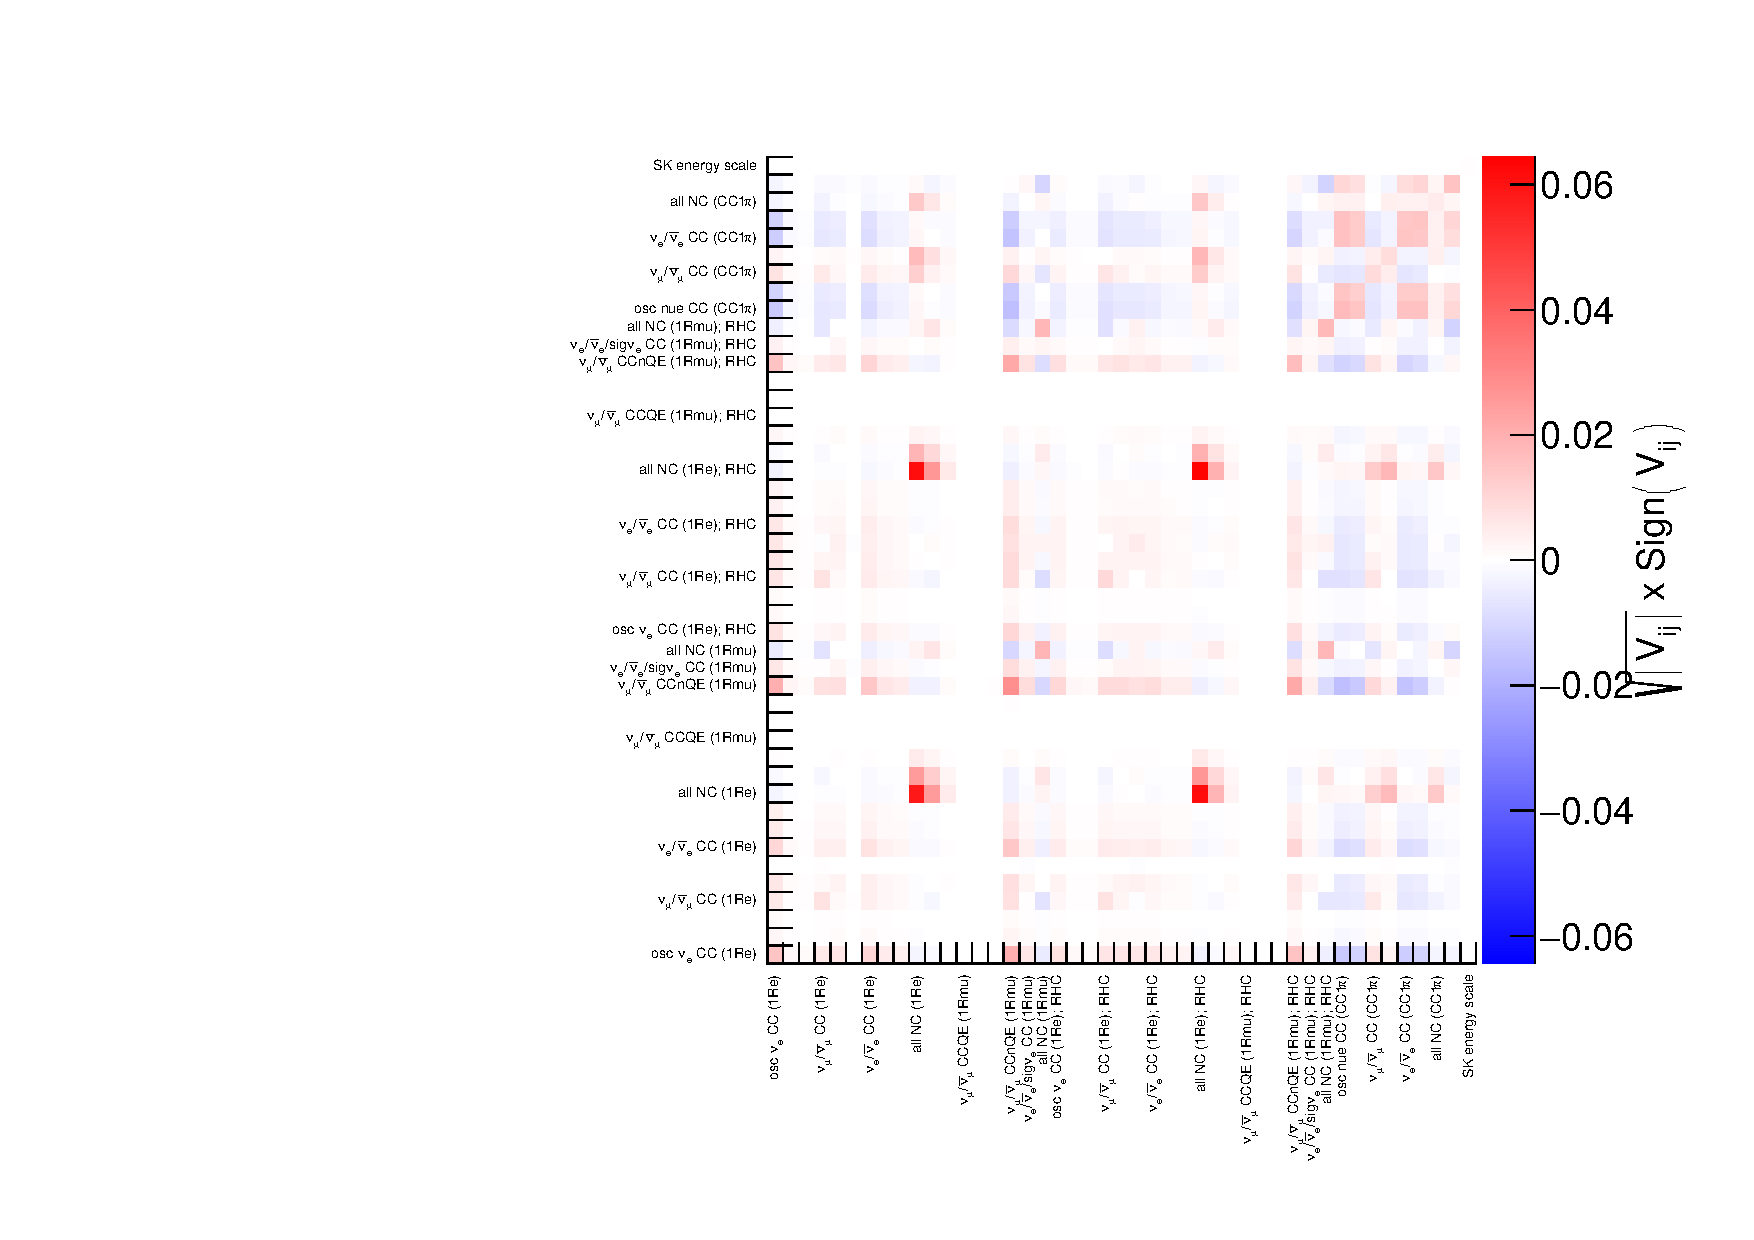
\includegraphics[width=\textwidth]{images/skdetfsi/skmatrix_fsi}
	\end{subfigure}
	\caption{The SK detector (top) and SK FSI+SI+PN (bottom) covariance matrices, with the values shown as the sign of the element times the square root of the absolute value of the element. Note that $z$ scaling is different in the two plots.}
	\label{fig:sk_corr}
\end{figure*}

\FloatBarrier
\clearpage

\subsection{Oscillation parameters and mass hierarchy (7 parameters)}

The 3-flavour oscillation probability is used.  All the nuisance oscillation parameters, i.e. those parameters which are not shown in a given contour, are marginalised except the mass hierarchy, which is fixed to either normal or inverted hierarchy.

For $\sin^2 \theta_{13}$ two different priors can be used, depending on whether the reactor constraint is applied, denoted as ``reactors", when applied and ``T2K only" when not applied.

\begin{table}[h]
	\centering
	\begin{tabular}{| c | c | c | c |}
 	\hline
Parameter(s)	& Prior		& Range    \\
\hline
$\sin^{2}\theta_{23}$	&  uniform 	& $[0.3; 0.7]$      \\
$\sin^{2} 2 \theta_{13}$ reactors		&  gaussian 		& $0.0830 \pm 0.0031$ 	\\
$\sin^{2} 2 \theta_{13}$ T2K only	   	&  uniform		& $[0.03; 0.2]$ 	\\
$\sin^{2} 2 \theta_{12}$  								&  gaussian 		& $0.851 \pm 0.020$ \\
$|$\dmsqtwothree$|$ (NH) / $|$\dmsqonethree$|$ (IH)      		&  uniform		& $ [2.3; 2.7] \times 10^{-3}~\mbox{eV}^2/\mbox{c}^4$		 \\
$\Delta m^{2}_{21}$      								&  gaussian 		& $(7.53 \pm 0.18) \times 10^{-5}~\mbox{eV}^2/\mbox{c}^4$		\\
$\delta_{CP}$                                               				&  uniform 	& $[-\pi; +\pi]$ \\
Mass Hierarchy										&  fixed 		& NH or IH \\  
\hline
\end{tabular}
\caption{
Treatment of the oscillation parameters in the $\nu/\bar{\nu}$ joint analysis. All the gaussian priors are from \cite{pdg_2014}. The parameter $\sin^{2} 2 \theta_{13}$ can be constrained with the measurement of reactor experiments using the gaussian prior, otherwise a uniform prior is used and the measurement relies only on the T2K data. The nominal values of $\sin^2 2 \theta_{13}$, $\sin^2 2 \theta_{12}$ and $\Delta m^2_{21}$ are from \cite{pdg_2014}, while all the other oscillation parameter values corresponds to the most probable values obtained by the Bayesian analysis on the T2K run 1-4 neutrino mode data \cite{T2KLongPaper}. The mass hierarchy is not marginalised but fixed to either NH or IH.
}
\label{tab:osc_param_priors}
\end{table}
\color{black}

\subsection{Systematic error on Super-K predictions}
\label{sec:systematics:errortables}

The effect of each category of systematic parameter on the expected event rate for Super-K sample is given in \cref{tab:sk_errors_summary}. The mean and RMS of \NumToysSmall throws of the respective systematics (with correlations taken into account) is computed for each sample and in the case of pre-BANFF and post-BANFF errors. When not measuring the effect of oscillation parameters variations, the oscillation parameters are fixed at Asimov A values (see \cref{sec:asimov_definition}).

For the measurement of $\delta_{CP}$ it is important to understand the effect of the systematic uncertainties on the ratio of the number of events between neutrino and antineutrino mode samples. If correlations do not reproduce the physics correctly, a fake asymmetry between neutrino and antineutrino oscillations can be seen. Furthermore, if correlations exist but are not taken into account, the measurement of $\delta_{CP}$ could be biased. The true value of $\delta_{CP}$ determines whether correlations or anti-correlations between systematic parameters have the greatest effect in hiding any oscillation asymmetry. In particular, if true $\delta_{CP} = \pm \pi/2$ then anti-correlation in the $e$-like samples could hide any oscillation asymmetry. Alternatively, in the case that true $\delta_{CP} \sim 0$ it is uncorrelated parameters that reduce the sensitivity to $\delta_{CP}$. The uncertainties on the ratios between neutrino and antineutrino mode events due to the systematic parameters are shown in \cref{tab:sk_errors_summary}. The most critical systematic parameters are $\sigma_{\nu_e}$ and $\sigma_{\bar{\nu}_e}$ which are applied respectively to $\nu_e$ and $\bar{\nu}_e$ events. Their fractional error from the BANFF covariance matrix is $\sim2.8$\% (see \cref{tab:sys_xsec_err}) and they are partially anti-correlated with non-diagonal elements in the covariance matrix of -0.0004.

It can be seen in \crefrange{tab:sk_errors_1Rmu}{tab:sk_errors_MultiRe} (\Cref{app:systematics}) that the reduction in the error on flux and constrained cross-section systematics achieved through the BANFF fit reduces the fractional error due to all systematics from $\sim 15\%$ to $\sim 5\%$ and $\sim 13\%$ to $\sim 4\%$ in the neutrino- and antineutrino-mode $\mu$-like samples respectively, from $\sim 17\%$ to $\sim 9\%$ and $\sim 14\%$ to $\sim 7\%$ in the neutrino- and antineutrino-mode $e$-like samples respectively, and from $\sim 22\%$ to $\sim 18\%$ in the \nueCConepi{}-like sample.

\begin{table}[H]
	\centering
	\begin{tabular}{|l||l|l||l|l|l|l|l|}
		\hline
		& \multicolumn{2}{c||}{\textbf{1-Ring $\mu$}} & \multicolumn{4}{c|}{\textbf{1-Ring $e$}} \\ \hline
		Error source & FHC & RHC & FHC & RHC & FHC 1 d.e. & FHC/RHC \\ \hline\hline
		SK Detector & 2.40 & 2.01 & 2.83 & 3.80 & 13.15 & 1.47 \\ \hline
		SK FSI+SI+PN & 2.21 & 1.98 & 3.00 & 2.31 & 11.43 & 1.57 \\ \hline
		Flux + Xsec constrained & 3.27 & 2.94 & 3.24 & 3.10 & 4.09 & 2.67 \\ \hline
		E$_\text{b}$ & 2.38 & 1.72 & 7.13 & 3.66 & 2.95 & 3.62 \\ \hline
		$\sigma(\nu_e)/\sigma(\bar{\nu}_e)$ & 0.00 & 0.00 & 2.63 & 1.46 & 2.61 & 3.03 \\ \hline
		NC1$\gamma$ & 0.00 & 0.00 & 1.09 & 2.60 & 0.33 & 1.50 \\ \hline
		NC Other & 0.25 & 0.25 & 0.15 & 0.33 & 0.99 & 0.18 \\ \hline
		Osc & 0.03 & 0.03 & 2.69 & 2.49 & 2.63 & 0.77 \\ \hline\hline
		All Systematics & 5.12 & 4.45 & 8.81 & 7.13 & 18.38 & 5.96 \\ \hline
		All with osc & 5.12 & 4.45 & 9.19 & 7.57 & 18.51 & 6.03 \\ \hline
	\end{tabular}
	\caption
	{
	Percentage error on event rate by error source and sample. Final column is the percentage error on the ratio of FHC/RHC events in the one-ring $e$ sample.
	}
	\label{tab:sk_errors_summary}
\end{table}


The error envelopes corresponding to \cref{tab:sk_errors_summary} are shown in \cref{app:systematics}.

\clearpage


%..................

%%% Local Variables:
%%% mode: latex
%%% TeX-master: "../TN327"
%%% End:
